
%------------------------------------------------

\section{Distribution}\index{distribution}
\label{sec:distr}

\subsection{Bernoulli distribution}\index{Bernoulli distribution}
\label{subsec:Bernoulli_distr}

The distribution is expressed by:

\begin{equation}\label{eq:Bernoulli_distr}
	f(k ; p) = \left\{
	\begin{array}{lcl}
		p     & & {\textrm{if } k = 1}\\
		1 - p & & {\textrm{if } k = 0}
	\end{array} \right.
	= p^{k}(1-p)^{1 - k} \quad \textrm{for } k \in \{ 0, 1 \}
\end{equation}

\begin{itemize}
	\item Mean: $\bar{x} = \sum_{x = 0}^{1} {x f(x ; p)}  = 1 \cdot f(1 ; p) = p$
	\item $\left \langle x^{2} \right \rangle = p$
	\item Variance: $\mathrm{V} = \left \langle x^{2} \right \rangle - {\bar{x}}^{2} = p(1 - p)$
\end{itemize}

\subsection{Binomial distribution}\index{binomial distribution}
\label{subsec:binomial_distr}

\begin{equation}\label{eq:binomial_distr}
	P(k ; n, p) = \frac{n!}{k!(n-k)!} p^{k}(1-p)^{n - k}
\end{equation}

\begin{itemize}
	\item Mean: $\bar{k} = np$
	\item Variance: $\mathrm{V} = np(1 - p)$
\end{itemize}

\newthought{Exercise}: \nameref{exer:binomial_distr}.

\subsection{Multinomial distribution}\index{multinomial distribution}
\label{subsec:multinomial_distr}

\marginnote{An example of multinomial distribution is a histogram containing $n$ entries distributed in $m$ bins.}

\begin{equation}\label{eq:multinomial_distr}
	P(k_{1}, k_{2}, \cdots, k_{m} ; n, p_{1}, \cdots, p_{m}) 
	= \frac{n!}{k_{1}! \cdots k_{m}!} {p_{1}}^{k_{1}} {p_{2}}^{k_{2}} \cdots {p_{m}}^{k_{m}}
\end{equation}

\begin{itemize}
	\item Average: $\overline{k_{i}} = n {p}_{i}$
	\item Variance: $\mathrm{V}\left[ k_{i} \right] = n {p}_{i} (1 - {p}_{i})$
	\item Covariance: $\mathrm{cov}\left( k_{i}, k_{j} \right) = - n {p}_{i} {p}_{j} \quad \forall i \neq j$
\end{itemize}

\subsection{Uniform distribution}\index{uniform distribution}
\label{subsec:uniform_distr}

A variable $x$ is uniformly distributed in the interval $[a, b)$, if its PDF (Figure~\ref{fig:CDF_PDF_uniform}) is constant in such range, \ie:

\begin{equation}\label{eq:uniform_distr}
	f(x) = \left\{
	\begin{array}{ccl}
		\frac{1}{b - a} & & {\textrm{if } a \leq x < b}\\
		0 & & {\textrm{otherwise}}
	\end{array} \right.
\end{equation}

\begin{figure}
	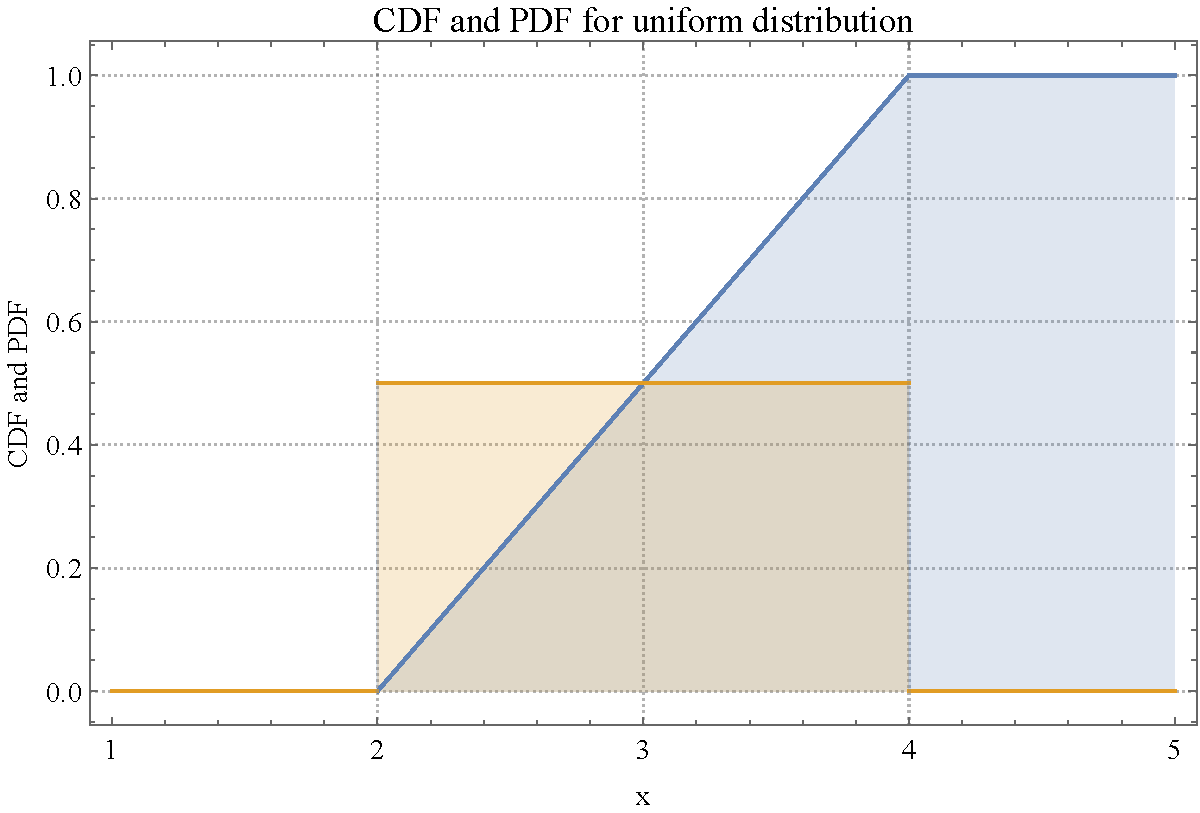
\includegraphics{probability/CDF_PDF_uniform.pdf}
	\caption[CDF and PDF for uniform distribution.][6pt]{CDF and PDF for uniform distribution.}
	\label{fig:CDF_PDF_uniform}
\end{figure}

\begin{itemize}
	\item Average: $\bar{x} = \frac{a + b}{2}$
	\item Standard deviation: $\sigma = \frac{b - a}{\sqrt{12}}$
\end{itemize}

\subsection{Exponential distribution}\index{exponential distribution}
\label{subsec:expo_distr}

Take a variable $x \geq 0$, and a constant $\lambda > 0$.

An exponential distribution (Figure~\ref{fig:CDF_PDF_expo}) has the form:

\begin{equation}\label{eq:expo_distr}
	f(x ; \lambda) = \lambda \mathrm{e}^{- \lambda x}
\end{equation}

\begin{figure}
	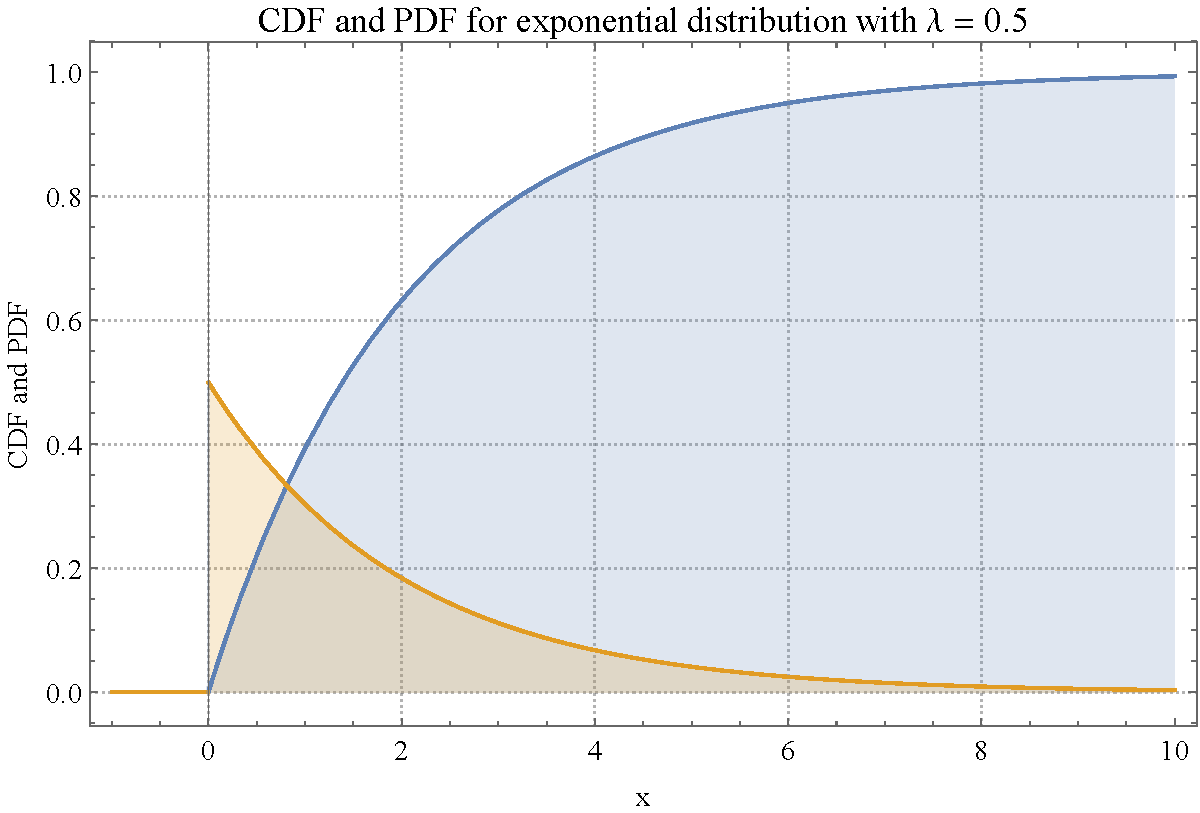
\includegraphics{probability/CDF_PDF_expo.pdf}
	\caption[CDF and PDF for exponential distribution.][6pt]{CDF and PDF for exponential distribution with $\lambda = 0.5$.}
	\label{fig:CDF_PDF_expo}
\end{figure}

\begin{itemize}
	\item Average: $\bar{x} = \frac{1}{\lambda}$
	\item Standard deviation: $\sigma = \frac{1}{\lambda}$
\end{itemize}

\newthought{Exercise}: \nameref{exer:expo_from_uniform}!

\subsection{Poisson distribution}\index{Poisson distribution}
\label{subsec:poisson_distr}

Consider a uniformly distributed variable $t$ over an interval $[0, \Delta t]$.

\marginnote{$t$ could be a space or a time variable, like the coordinate of some particle bit on a pixelated detector, or the time of arrival of some particles.}

Assume $t$ is extracted $n$ times in $\Delta t$, the rate of extractions is $r = \frac{n}{\Delta t}$.

Let's consider only the extractions $k$ in a shorter interval $\delta t$, which are clearly binomial distributed. 

Assume $n$ and $\Delta t$ are constant, and take the limits $n \to \infty$ and $\Delta t \to \infty$, keeping their ratio $r$ fixed.

The expected value $\nu$ of the number of extractions in $\delta t$ is:

$$
\nu = \left \langle k \right \rangle = \frac{n}{\Delta t} \delta t = r \delta t
$$

And $k$ follows a binomial:

$$
P(k ; n, \nu) = \frac{n!}{k!(n-k)!} {\left( \frac{\nu}{n} \right)}^{k} {\left( 1 - \frac{\nu}{n} \right)}^{n - k}
$$

with $\lim_{n \to \infty}$:

$$
P(k ; n, \nu) 
= \frac{\nu^{k}}{k!} 
\cdot \underset{\to 1}{\underbrace{\frac{n(n - 1) \cdots (n - k + 1)}{n^{k}}}}  
\cdot \underset{\to \mathrm{e}^{- \nu}}{\underbrace{{\left( 1 - \frac{\nu}{n} \right)}^{n}}} 
\cdot \underset{\to 1}{\underbrace{{\left( 1 - \frac{\nu}{n} \right)}^{- k}}}
$$

We have then the Poisson distribution:

\begin{equation}\label{eq:poisson_distr}
	P(k ; \nu) = \frac{\nu^{k} \mathrm{e}^{- \nu}}{k!}
\end{equation} 

\begin{itemize}
	\item Average: $\bar{k} = \nu$
	\item Standard deviation: $\sigma = \sqrt{\nu}$
\end{itemize}

\newthought{Exercise}: \nameref{exer:poisson_distr}.

\subsection{Properties of Poisson distribution}\index{Poisson distribution!property}
\label{subsec:prop_of_poisson_distr}

\begin{itemize}
	\item For large $\nu$, a Poisson distribution can be approximated with a Gaussian\index{Gaussian distribution} with $\mu = \nu$ and $\sigma = \sqrt{\nu}$.
	\item A binomial distribution\index{binomial distribution} with $p \ll 1$ can be approximated with a Poisson distribution with $\nu = np$.
	\item If two variables $k_{1}$ and $k_{2}$ are Poisson distributed with expectation values $\nu_{1}$ and $\nu_{2}$, their sum $k = k_{1} + k_{2}$ is Poisson distributed with expectation value $\nu = \nu_{1} + \nu_{2}$. (Figure~\ref{fig:prop_of_Poisson_distr}) 
		\marginnote[-6pt]{This can be expanded to any number of Poisson variables.}
	\item Randomly picking with probability $\varepsilon$ from a Poisson process gives again a Poisson process.
		\marginnote[-6pt]{This is the case of a detector with efficiency $\varepsilon$, which measures a Poisson process with expectation value $\nu_{0}$!}
		\begin{description}
			\item Take a Poisson variable $n_{0}$ with expectation value $\nu_{0}$. 
			\item Then a binomial variable $k$ with probability $\varepsilon$ and sample size $n_{0}$ is distributed as a Poisson with average $\nu = \varepsilon \nu_{0}$.
		\end{description}
\end{itemize}

\begin{figure}
	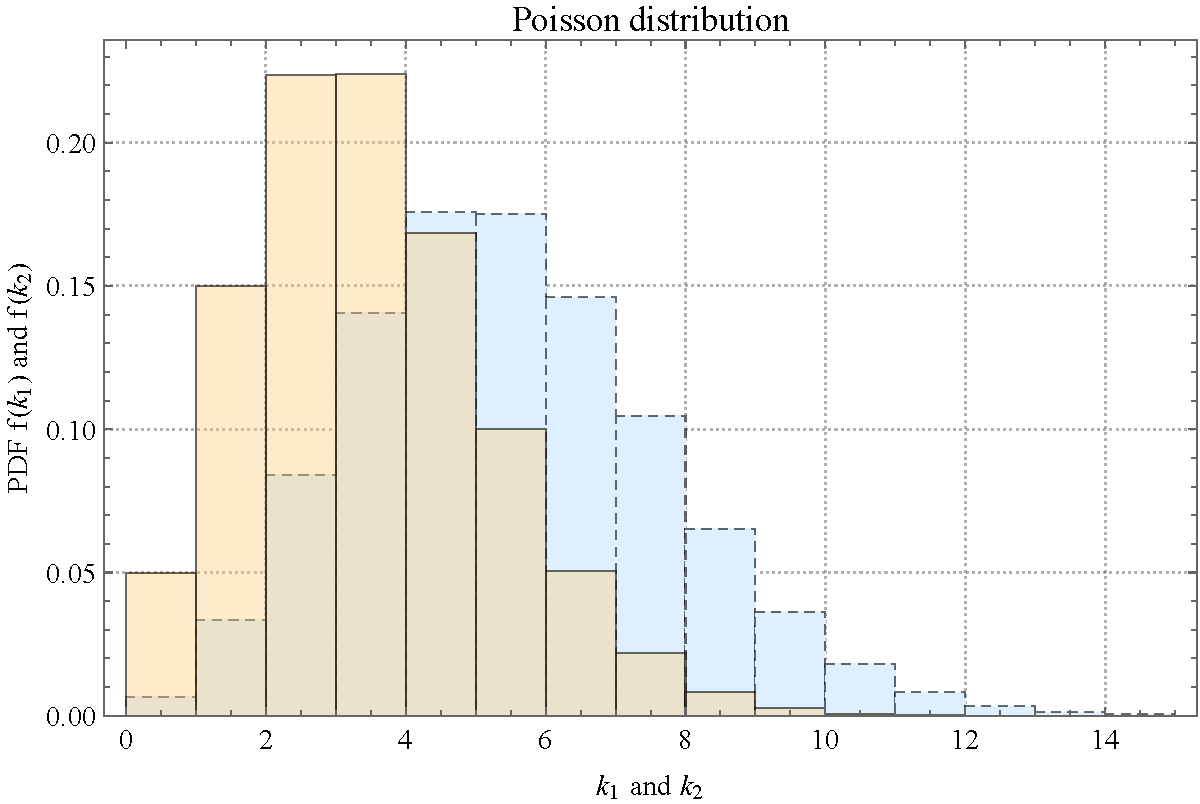
\includegraphics{probability/prop_of_Poisson_distr.pdf}
	\caption[PDF for two Poisson distributions.][6pt]{PDF for two Poisson distributions.}
	\label{fig:prop_of_Poisson_distr}
\end{figure}

\newthought{Examples}:

Suppose you have $n$ unstable isotopes, with decay rate $\lambda$ (numbers of decays per unit time).

In a time $\Delta t$, the probability of a decay is $p = \lambda t$.

The distribution of the numbers of decayed nuclei in a time $\Delta t$ is:

\begin{enumerate}
	\item Binomial, if $p \gtrsim 0.1$
	\item Poisson, if $p \lesssim 0.1$
\end{enumerate}

\begin{table}
	\centering
	\begin{tabular}{l c c}
		\toprule
		& ${}^{137}\mathrm{Cs}$ & ${}^{82}\mathrm{Rb}$\\
		\midrule
		Decay mode 
		& $\beta -$ & EC $\beta +$\\
		Half-life $T_{1/2}$ 
		& $\unit[30.08]{y}$ & $\unit[75.45]{s}$\\
		Decay rate $\lambda$ $[\unit{s}^{-1}]$ 
		& $7.3 \times 10^{-10}$ & $9.2 \times 10^{-3}$\\
		Radioactive activity $A$ $[\unit{Ci}]$ 
		& $1 \mu \unit{Ci}$ & $\unit[1]{m Ci}$\\
		Radioactive activity $A$ $[\unit{Bq}]$ 
		& $3.7 \times 10^{4}$ & $3.7 \times 10^{7}$\\
		\tabincell{l}{Initial amount of active substance \\ $N_{0} = \frac{A}{\lambda}$} & $5.1 \times 10^{13}$   & $4 \times 10^{9}$      \\
		\tabincell{l}{Number of decay events in 1 hour \\ $\Delta N = N_{0} \times \lambda \times \Delta t$} & $1.3 \times 10^{8} \ll N_{0}$ & $1.3 \times 10^{11} {\color{Red} > N_{0}}$\\
		\bottomrule
	\end{tabular}
	\caption[Binomial or Poisson?]{Binomial or Poisson for measuring decays over 1 hour?}
	\label{tab:binomial_or_poisson}
\end{table}

\subsection{Normal (Gaussian) distribution}\index{Gaussian distribution}
\label{subsec:gaussian_distr}

\begin{equation}\label{eq:gaussian_distr}
	g(x ; \mu, \sigma) = \frac{1}{\sigma \sqrt{2 \pi}} 
	\mathrm{e}^{- \frac{1}{2} {\left( \frac{x - \mu}{\sigma} \right)}^{2}}
\end{equation}

with $x$ continuous. 

For $\mu = 0$ and $\sigma = 1$, we have a standard normal distribution\index{standard normal distribution}:

\begin{equation}\label{eq:std_normal_distr}
	\phi(x) = \frac{1}{\sqrt{2 \pi}} \mathrm{e}^{- \frac{x^{2}}{2}}
\end{equation}

\begin{itemize}
	\item Mean: $\mu$
	\item Standard deviation: $\sigma$
\end{itemize}

Cumulative of standard normal:

\begin{equation}\label{eq:cdf_std_normal}
	\Phi(x) = \frac{1}{\sqrt{2 \pi}} \int_{-\infty}^{x} \mathrm{e}^{- \frac{y^{2}}{2}} \,\mathrm{d}y 
	= \frac{1}{2} \left[ \mathrm{erf}\left( \frac{x}{\sqrt{2}} \right) + 1 \right]
\end{equation}

Cumulative of Gaussian:

\begin{equation}\label{eq:cdf_Gaussian}
	G(x ; \mu, \sigma) = \Phi \left( \frac{x - \mu}{\sigma} \right) 
	= \frac{1}{2} \left[ \mathrm{erf}\left( \frac{x - \mu}{\sigma \sqrt{2}} \right) + 1 \right]
\end{equation}

\subsection{Properties of Gaussian distribution}\index{Gaussian distribution!property}
\label{subsec:prop_of_gaussian_distr}

If $x_{1}$ and $x_{2}$ are Gaussian distributed with means $\mu_{1}$, $\mu_{2}$ and standard deviations $\sigma_{1}$, $\sigma_{2}$, their combination $x = a{x}_{1} + b{x}_{2}$ is Gaussian distributed with mean $\mu = a{\mu}_{1} + b{\mu}_{2}$ and standard deviation $\sigma = \sqrt{a^{2}{{\sigma}_{1}}^{2} + b^{2}{{\sigma}_{2}}^{2}}$.

\marginnote[-6pt]{Sometimes the sum of two Gaussian distributed variables is not a Gaussian! \nameref{exer:sum_of_Gaussian}.}

\subsection{Multivariate normal distribution}\index{multivariate normal distribution}
\label{subsec:multivariate_normal_distr}

A multivariate normal distribution is a Gaussian in dim > 1.

\paragraph{Dim = 2}

\begin{equation}\label{eq:bivariate_normal_joint_density}
	g(x, y) = \frac{1}{\sqrt{2 \pi {\left| C \right|}}} \mathrm{e}^{\left[ - \frac{1}{2} (x, y) C^{-1} 
	\left( \begin{array}{c}
		x \\
		y 
	\end{array} \right) \right]}
\end{equation}

where $C$ is the covariance matrix\index{covariance matrix}: 

\begin{equation}\label{eq:covariance_matrix}
	C = 
	\left( \begin{array}{cc}
		{\sigma_{x}}^{2} & \rho_{xy} \sigma_{x} \sigma_{y} \\
		\rho_{xy} \sigma_{x} \sigma_{y} & {\sigma_{y}}^{2}
	\end{array} \right)
\end{equation}

One can also forget about the covariance matrix and define a rotation of the system of reference: 

\begin{equation}\label{eq:rotation_of_system_of_reference}
	\left\{
	\begin{array}{l}
		x' = \cos \phi \cdot x + \sin \phi \cdot y\\
		y' = - \sin \phi \cdot x + \cos \phi \cdot y
	\end{array} \right.
\end{equation}

therefore, 

\begin{equation}
	g(x', y') = \frac{1}{2 \pi \sigma_{1} \sigma_{2}} 
	\mathrm{e}^{- \frac{1}{2} {\left( \frac{x' - \mu_{1}}{\sigma_{1}} \right)}^{2}} 
	\mathrm{e}^{- \frac{1}{2} {\left( \frac{y' - \mu_{2}}{\sigma_{2}} \right)}^{2}}
\end{equation}

\marginnote[-6pt]{By importing the rotation, one can get rid of the correlation.}

\paragraph{General formula for dim = $n$}

\begin{equation}\label{eq:bivariate_normal_joint_density}
	g(\vec{x}) = \frac{1}{\sqrt{(2 \pi)^{n} {\left| C \right|}}} 
	\mathrm{e}^{\left[ - \frac{1}{2} (\vec{x} - \vec{\mu})^{T} C^{-1} (\vec{x} - \vec{\mu}) \right]}
\end{equation}

\subsection{Chi-square distribution}\index{chi-square distribution}
\label{subsec:chisquare_distr}

A $\chi^{2}$ random variable with $n$ degrees of freedom is the sum of $n$ standard normal variables.

\begin{equation}\label{eq:chisquare_distr}
	f(\chi^{2} ; n) = \frac{2^{- \frac{n}{2}}}{\Gamma(\frac{n}{2})} \chi^{n - 2} \mathrm{e}^{- \frac{\chi^{2}}{2}}
\end{equation}

where $\Gamma$ is the gamma function\index{gamma function}, which is the extension of the factorial\index{factorial}.

\marginnote[-6pt]{For integer, $\Gamma(n) = (n -1)!$ .}

\begin{itemize}
	\item Expectation value: $\left \langle \chi^{2} \right \rangle = n$
	\item Standard deviation: $\sigma = \sqrt{2n}$
\end{itemize}

\newthought{Exercise}: \nameref{exer:chisquare_distr}.
